\section{Résultats des simulations sur \textsc{Aspen Plus}}
\label{sec:aspen_simulation}

Nous regroupons dans les figures~\ref{fig:RK-ASPEN} à~\ref{fig:SRK,750,270,1}
tous les résultats produits par nos simulations réalisées sur \textsc{Aspen Plus}. 
Pour chacune d'elles, nous précisons le modèle utilisé,
les conditions de température et de pression dans le réacteur 
et la fraction purgée du recyclage. 
On accorde en particulier de l'attention aux résultats 
concernant les deux flux suivants: \textsc{nh3,out} et \textsc{purge}.

\begin{figure}[h!]
	\begin{center}
		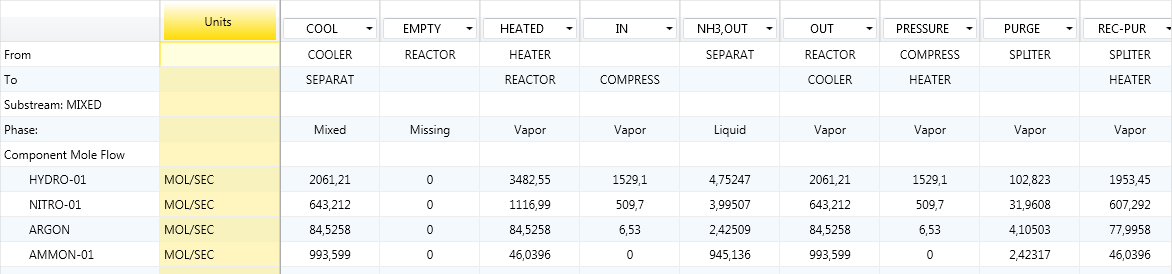
\includegraphics[scale=0.5]{../tache2/img_aspen/RK-ASPEN.png}
	\end{center}
	\caption{Modèle \texttt{RK-ASPEN}, $750\si{\kelvin}$, $270\si{\bar}$, 5\%}
	\label{fig:RK-ASPEN}
\end{figure}

\begin{figure}[h!]
	\begin{center}
		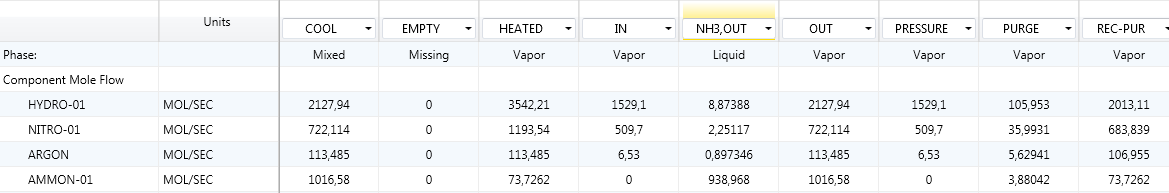
\includegraphics[scale=0.5]{../tache2/img_aspen/PSRK.png}
	\end{center}
	\caption{Modèle \texttt{PSRK}, $750\si{\kelvin}$, $270\si{\bar}$, 5\%}
	\label{fig:PSRK}
\end{figure}

\begin{figure}[h!]
	\begin{center}
		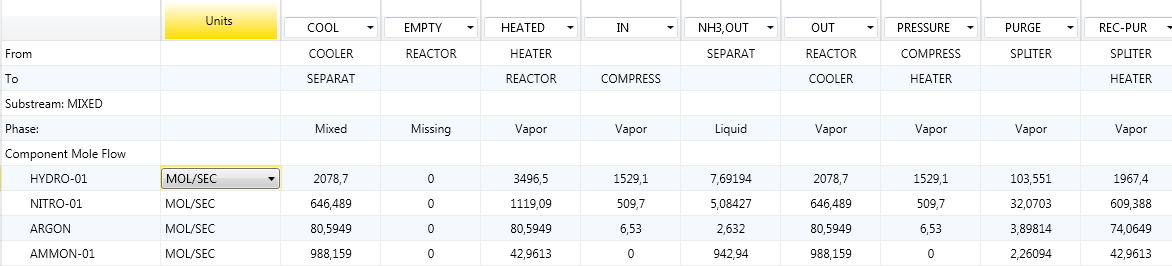
\includegraphics[scale=0.5]{../tache2/img_aspen/SRK,750,270,5.png}
	\end{center}
	\caption{Modèle \texttt{SRK}, $750\si{\kelvin}$, $270\si{\bar}$, 5\%}
	\label{fig:SRK,750,270,0.05}
\end{figure}

\begin{figure}[h!]
	\begin{center}
		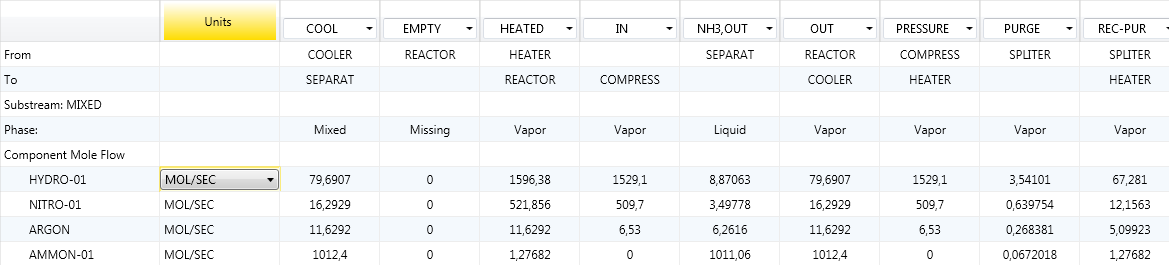
\includegraphics[scale=0.5]{../tache2/img_aspen/SRK,500,270.png}
	\end{center}
	\caption{Modèle \texttt{SRK}, $500\si{\kelvin}$, $270\si{\bar}$, 5\%}
	\label{fig:SRK,500,270,0.05}
\end{figure}

\begin{figure}[h!]
	\begin{center}
		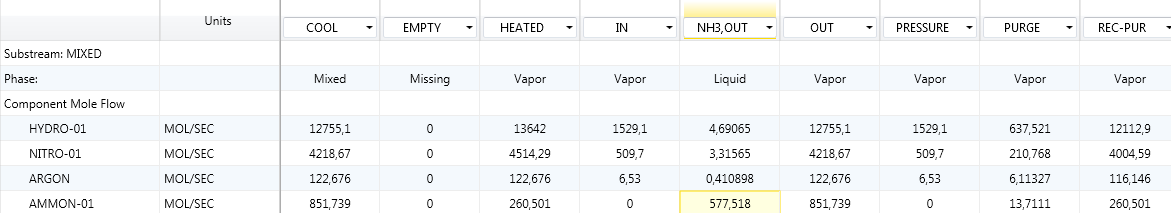
\includegraphics[scale=0.5]{../tache2/img_aspen/SRK,1000,270.png}
	\end{center}
	\caption{Modèle \texttt{SRK}, $1000\si{\kelvin}$, $270\si{\bar}$, 5\%}
	\label{fig:SRK,1000,270,0.05}
\end{figure}

\begin{figure}[h!]
	\begin{center}
		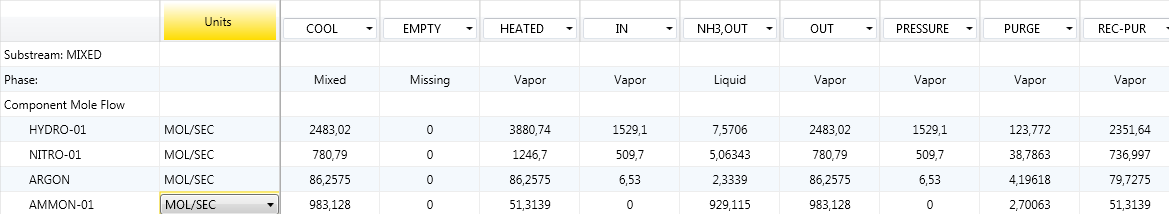
\includegraphics[scale=0.5]{../tache2/img_aspen/SRK,750,220.png}
	\end{center}
	\caption{Modèle \texttt{SRK}, $750\si{\kelvin}$, $220\si{\bar}$, 5\%}
	\label{fig:SRK,750,220,0.05}
\end{figure}

\begin{figure}[h!]
	\begin{center}
		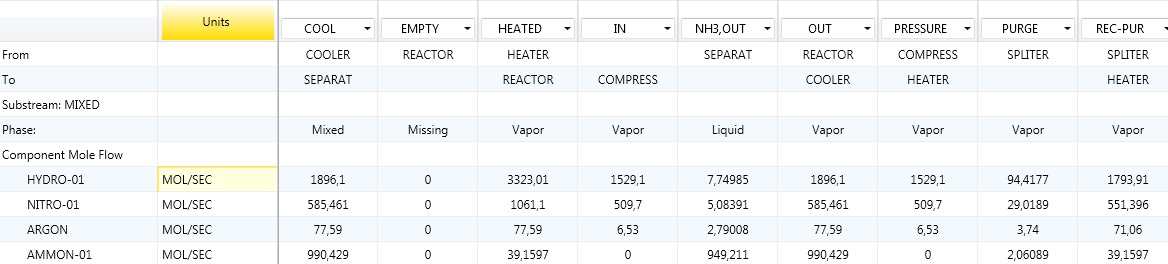
\includegraphics[scale=0.5]{../tache2/img_aspen/SRK,750,300.png}
	\end{center}
	\caption{Modèle \texttt{SRK}, $750\si{\kelvin}$, $300\si{\bar}$, 5\%}
	\label{fig:SRK,750,300,0.05}
\end{figure}

\begin{figure}[h!]
	\begin{center}
		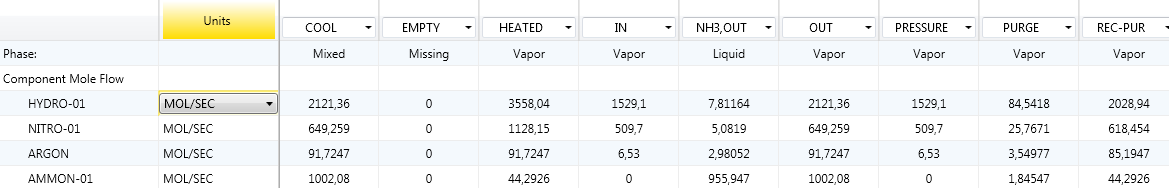
\includegraphics[scale=0.5]{../tache2/img_aspen/SRK,750,270,4.png}
	\end{center}
	\caption{Modèle \texttt{SRK}, $750\si{\kelvin}$, $270\si{\bar}$, 4\%}
	\label{fig:SRK,750,270,0.04}
\end{figure}

\begin{figure}[h!]
	\begin{center}
		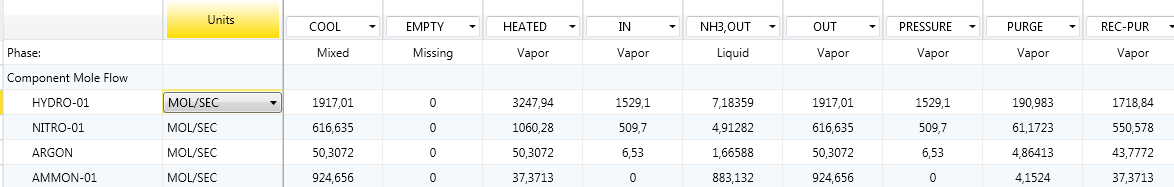
\includegraphics[scale=0.5]{../tache2/img_aspen/SRK,750,270,10.png}
	\end{center}
	\caption{Modèle \texttt{SRK}, $750\si{\kelvin}$, $270\si{\bar}$, 10\%}
	\label{fig:SRK,750,270,0.1}
\end{figure}

\begin{figure}[h!]
	\begin{center}
		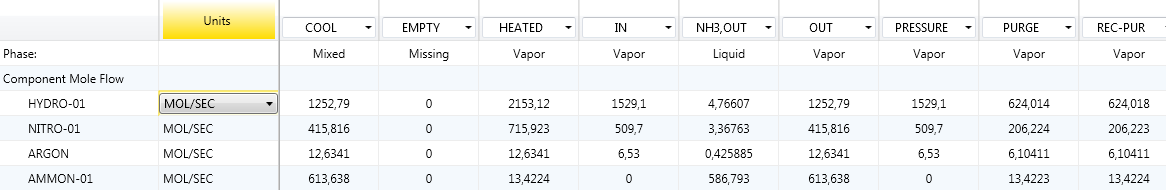
\includegraphics[scale=0.5]{../tache2/img_aspen/SRK,750,270,50.png}
	\end{center}
	\caption{Modèle \texttt{SRK}, $750\si{\kelvin}$, $270\si{\bar}$, 50\%}
	\label{fig:SRK,750,270,0.5}
\end{figure}

\begin{figure}[h!]
	\begin{center}
		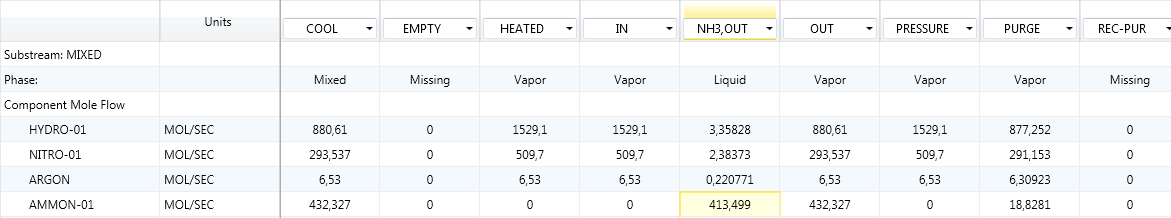
\includegraphics[scale=0.5]{../tache2/img_aspen/SRK,750,270,100.png}
	\end{center}
	\caption{Modèle \texttt{SRK}, $750\si{\kelvin}$, $270\si{\bar}$, 100\%}
	\label{fig:SRK,750,270,1}
\end{figure}

